\subsection{Анализ узкого места}

Код генерируемый EML работает по следующему принципу: для шаблона создается изначально пустой буфер.
Буфер является обычным динамическим массивом, подобным std::vector из C++.
Весь шаблонный HTML код преобразовывается в строчный литерал.
Эти строки поэтапно добавляются в буфер, формируя результат.
Между ними происходит исполнение OCaml кода, что и позволяет использовать EML для обработки произвольного шаблонного кода.

Была выдвинута гипотеза, заключающаяся в том что Dream EML показывает плохие результаты из-за большого количества аллокаций.
Дело в том что для сохранения чистоты функций, использующих EML, для каждого шаблона создается свой буфер для временных данных.
Эти аллокации, однако, не являются необходимыми и сразу же выкидываются после завершения исполнения функции.
Посему была предпринята попытка добавить пул из заранее аллоцированных буферов для рендеринга и заменить создание новых буферов на взятие их из пула.
EML является препроцессором и не добавляется в код приложений как зависимость, поэтому добавить общий рантайм для всех файлов проходящих через препроцессинг не представляется возможным.
В связи с этим, этот пул создавается в начале каждого файла, проходящего через препроцессинг.

Парсер EML работает в 3 этапа - токенизация, трансформация и генерация.
На первом этапе файл разбивается на токены 4 типов - code\_block - блоки кода, options - опции препроцессинга, newline - новые линии и template - HTML код шаблонов.
Основана токенизация на табуляции программы, либо на нескольких специальных символах.
На втором этапе выделенные содержимое токенов преобразовывается, например удаляются лишние пробелы в конце строк и объединяются последовательности одинаковых токенов.
Следом на последнем этапе токены заменяются на соответствующие конструкции в итоговом коде.

С учетом этого, для добавления такого пула было произведено два действия: был создан токен начала файла и был добавлен код, преобразующий этот токен в код создания пула - соответственно модификации для первого и последнего этапов.
На последнем этапе также были произведены модификации с учетом нового пула:
старый код создания локальных буферов был заменен на вызов функции получения буфера из пула;
вместо вызова функции получения текста из буфера был добавлен код возврата буфера в пул с его последующим очищением.
Пул сделан параметризируемым по размеру буфера и количеству буферов создаваемых на момент инициализации программы.
Параметры принимаются как аргументы запуска препроцессора: --buffer-size и --pool-size соответственно.

\subsection{Механизм пула буферов}

OCaml\footnote{Dream EML также поддерживает синтаксис Reason, для которого была написана своя реализация. Поскольку суть не меняется, в работе она не приводится.} код пула буферов, вставляемый в начале каждого файла выглядит следующим образом\footnote{
Поскольку создать общий рантайм или библиотеку не представляется возможным, дабы не вызвать конфликт имен, все имена функций были префиксированы с тремя нижними подчеркиваниями.}:

\begin{lstlisting}
let ___eml_pool = ref (
    List.init ___EML_POOL_SIZE 
    (fun _ -> Buffer.create ___EML_BUFFER_SIZE)
)
let ___eml_get_buffer pool =
    match !pool with
    | buf :: bufs ->
        pool := bufs;
        Buffer.clear buf;
        buf
    | [] -> Buffer.create ___EML_BUFFER_SIZE
let ___eml_return_buffer pool buf =
    pool := buf :: !pool;
    Buffer.contents buf
\end{lstlisting}

Поскольку OCaml имеет кооперативную модель многопоточности, весь пул представляет собой простой связанный список.
Секвенциальное исполнение кода гарантирует что за раз пул будет отдаваться только одному потоку.
Это позволяет не использовать механизмы синхронизации в его реализации.

\subsection{Результат оптимизации}

Также как и для сравнительного анализа, здесь был сделан тест с помощью секундомера и тест с помощью ocaml-benchmark.

Результаты первого теста приведены на графике \ref{fig:ratio}.
Для наглядности, на графике время работы старого и нового EML отнесено друг к другу.
В среднем производительность увеличилась в 2.65 раз.

\begin{figure}[h!]
    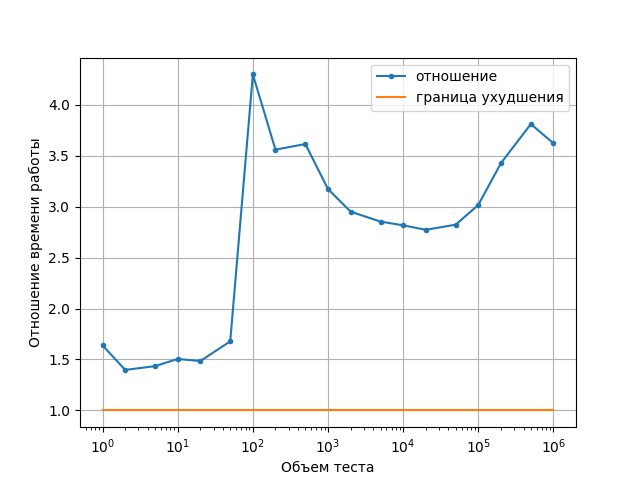
\includegraphics[width=\textwidth]{ratio.png}
    \caption{Результат оптимизации пула буферов. Построен с помощью matplotlib. Показано отношение времени работы до оптимизации к времени после. Граница ухудшения - значение отношения равное 1, что соответствует границе после которой считается что скорость увеличилась.}
    \label{fig:ratio}
\end{figure}

Результаты второго теста приведены на рисунке \ref{fig:optimised}.
Количество major аллокаций в новом EML значительно уменьшилось по сравнению со старым.
Во многих случаях major аллокации вообще не осуществлялись, что выгодно выделяет EML на фоне остальных фреймворков.



\subsection{Дополнительный анализ}


В связи с этим чаще всего, для простых серверов достаточно будет иметь всего 1 буфер в этом пуле, который постоянно переиспользуется.
По умолчанию создается всего 1 буфер размером 4096 символов.
Эти настройки не являются оптимальными для всех страниц, однако являются достаточно гибкими для большинства страниц.
Страницы, имеющие большой объем текста, могут создавать меньшее количество буферов с большим размером.
% Эта настрйока релевантна для страниц, имеющих обратную проблему - малое количество рендерингов большого объема. % // TODO: сделать бенчмарк доказывающий это утверждение должно быть несложно
Подобная гибкость в настройке не предоставляется другими решениями, что выделяет EML как уникальный инструмент.


